\documentclass{article}
\usepackage[a4paper,margin=1in]{geometry}
\usepackage{amsmath, amsfonts, amssymb, amstext, mathtools, stmaryrd, textcomp, xcolor, graphicx, tikz}
\usepackage[hidelinks]{hyperref}
\usetikzlibrary{automata, positioning, arrows, trees}
\tikzset{->,>=stealth,
every state/.style={thick, fill=gray!10}, 
initial text=$ $,
}
\newcommand{\e}{\varepsilon}
\newcommand{\s}{\Sigma}
\newcommand{\g}{\Gamma}
\newcommand{\so}{\rightarrow}
\newcommand{\str}{\texttt}
\newcommand{\newp}{\\[2mm]}
\newcommand{\defeq}{\coloneqq}

\title{Homework 04}
\author{Aaron Wang}
\date{February 21 2025}

\begin{document}
\maketitle
\begin{enumerate}
    \item \textbf{Arithmetic expressions}. Consider the grammar $G_4$ (page 105) for arithmetic expressions, with start symbol $E$:
    \begin{align*}
        & E \rightarrow E \: \str{+} \: T \: | \: T\\
        & T \rightarrow T \: \str{*} \: F \: | \: F\\
        & F \rightarrow \str{(}E\str{)} \: | \: \str{a} \: | \: \str{b} \: | \: \str{c}
    \end{align*}
    \begin{enumerate}
        \item [(a)][cf. Exercise 2.1] Give derivations for the following strings. You may write them either as a sequence of rewrites $(E \implies \cdots)$ or as a tree.
        \begin{enumerate}
            \item \str{a + b + c}
            \item \str{a * b + c}
            \item \str{a * (b + c)}
        \end{enumerate}
        
\textcolor{red}{
\begin{center}
\begin{minipage}{0.25\textwidth}
    i.
    \begin{center}
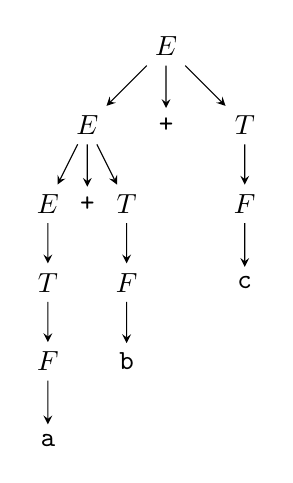
\begin{tikzpicture}[
    level distance=1cm,
    level 1/.style={sibling distance=1cm},
    level 2/.style={sibling distance=0.5cm}
]
    \node {$E$}
    child {node {$E$}
        child {node {$E$}
            child {node {$T$}
                child {node {$F$}
                    child {node {\str{a}}
                    }
                }
            }
        }
        child {node {\str{+}}}
        child {node {$T$}
            child {node {$F$}
                child {node {\str{b}}
                }
            }
        }
    }
    child {node {\str{+}}}
    child {node {$T$}
        child {node {$F$}
            child {node {\str{c}}}
        }
    };
\end{tikzpicture}
\end{center}
\end{minipage}
\begin{minipage}{0.25\textwidth}
    ii.
    \begin{center}
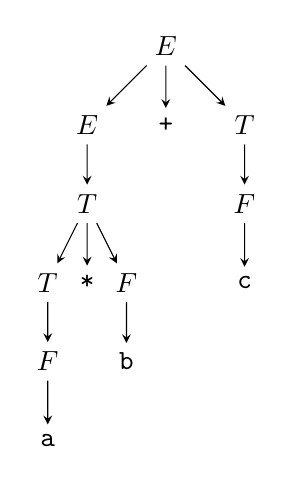
\begin{tikzpicture}[
    level distance=1cm,
    level 1/.style={sibling distance=1cm},
    level 2/.style={sibling distance=0.5cm}
]
    \node {$E$}
    child {node {$E$}
        child {node{$T$}
            child {node{$T$}
                child{node{$F$}
                    child{node{\str{a}}}
                }
            }
            child {node{\str{*}}}
            child {node{$F$}
                child{node {\str{b}}}
            }
        }
    }
    child {node {\str{+}}}
    child {node {$T$}
        child {node {$F$}
            child {node {\str{c}}}
        }
    };
\end{tikzpicture}
\end{center}
\end{minipage}
\begin{minipage}{0.25\textwidth}
    iii.
    \begin{center}
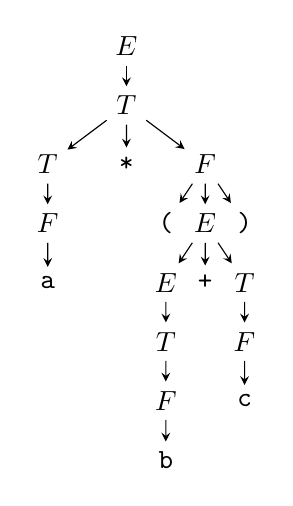
\begin{tikzpicture}[
    level distance=0.75cm,
    level 2/.style={sibling distance=1cm},
    level 3/.style={sibling distance=0.5cm}
]
    \node {$E$}
    child {node {$T$}
        child {node {$T$}
            child {node{$F$}
                child{node{\str{a}}}
            }
        }
        child {node {\str{*}}}
        child {node {$F$}
            child {node{\str{(}}}
            child {node {$E$}
                child {node {$E$}
                    child {node {$T$}
                        child {node{$F$}
                            child{node{\str{b}}}
                        }
                    }
                }
                child {node {\str{+}}}
                child {node {$T$}
                    child {node{$F$}
                        child{node{\str{c}}}
                    }
                }
            }
            child {node{\str{)}}}
        }
    };
\end{tikzpicture}
\end{center}
\end{minipage}
\end{center}
}

        \item [(b)]Modify $G_4$ to allow an exponentiation operator $\uparrow$.
        \begin{itemize}
            \item It should have \textit{higher precedence} than multiplication; that is, in the derivation of the string \str{a * b} $\uparrow$ \str{c}, there should be a nonterminal that rewrites to \str{b} $\uparrow$ \str{c}, and there should not be a nonterminal that rewrites to \str{a * b}.
            \item It should be (unlike \str{*} and \str{+}) \textit{right-associative}; that is, in the derivation of the string\\ \str{a} $\uparrow$ \str{b} $\uparrow$ \str{c}, there should be a nonterminal that rewrites to \str{b} $\uparrow$ \str{c}, and there should not be a nonterminal that rewrites to \str{a} $\uparrow$ \str{b}.
        \end{itemize}
        \textcolor{red}{
\begin{align*}
& E \rightarrow E \: \str{+} \: T \: | \: T\\
& T \rightarrow T \: \str{*} \: F \: | \: F\\
& F \rightarrow O \: \str{$\uparrow$} \: F \: | \: O\\
& O \rightarrow \str{(}E\str{)} \: | \: \str{a} \: | \: \str{b} \: | \: \str{c}
\end{align*}
}
    \end{enumerate}
    \item Write both a PDA and a CFG for the language (page 80):
    \[
    C = \big\{w \in \{0, 1\}^* | w\text{ has an equal number of \str{0}s and \str{1}s}\big\}.
    \]
    Please include a brief explanation of why they work. (If you design a PDA and then convert it to a CFG, your explanation for the CFG can simply be, ``I converted my PDA to a CFG,'' and similarly if you convert a CFG to a PDA.)\newp
    \answer{
The intuition for the following conversion is this. Use the 2 stacks in the same way as the tape would be used where the first stack is used to hold everything preceding the head and the other stack holds everything following and where the head is currently looking at the top element on the second stack. The head moves right by moving one element from the second stack to the first stack, and moves left by moving an element from the first stack to the second. 
To consider the edge case of moving left when all the way at the left already, you check for a $\$$ and in that case, you move back right.
To consider the edge case, where we extend pass the starting string (go to trailing spaces), we would
Let $M$ be a TM.\newp
Let $P = \{Q,\s,\g, \delta, s, F\}$ be the 2PDA such that
\begin{quote}
\begin{enumerate}
    \item [1.] The string ($\s$) alphabet is the same as that of $M$.
    \item [2.] $\g = \s \cup \{\text{\spc, \str{\$}}\}$. The stack alphabet is string alphabet with \spc \:and \str{\$}. 
    \item [3.] Have pre-processing states to read the input onto the stack and add \str{\$} to demarcate the end and beginning. $\forall a \in \s$.\footnote{The outgoing transition from $s_2$ will be $\e$, $\e$, $\e \rightarrow \e$, $\e$ into the original start state }
    \begin{figure}[h]
\centering
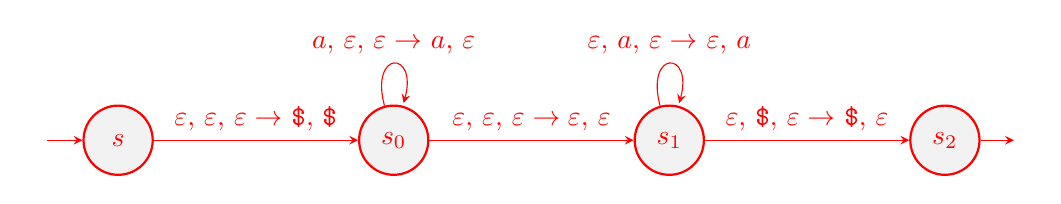
\begin{tikzpicture}
\color{red}
    \node[state, initial] (q0) {$s$};
    \node[state, xshift=3.5cm] (q1) {$s_0$};
    \node[state, xshift=7cm] (q2) {$s_1$};
    \node[state, xshift=10.5cm] (q3) {$s_2$};
    \node[draw=none, xshift=11.5cm] (phantom) {};

    \draw
    (q0) edge[] node[above]{$\e$, $\e$, $\e \rightarrow$ \str{\$}, \str{\$}}(q1)
    (q1) edge[loop above] node[above]{$a$, $\e$, $\e \rightarrow$ $a$, $\e$} (q1)
    (q1) edge[] node[above]{$\e$, $\e$, $\e \rightarrow \e$, $\e$}(q2)
    (q2) edge[loop above] node[above]{$\e$, $a$, $\e \rightarrow$ $\e$, $a$} (q2)
    (q2) edge[] node[above]{$\e$, \str{\$}, $\e \rightarrow$ \str{\$}, $\e$}(q3)
    (q3) edge[] node[above]{\:} (phantom)
    ;
\end{tikzpicture}
\end{figure}
    \item [4.] For each state $q$ of $M$, the same state $q$ in $P$.
    \begin{enumerate}
        \item $F = \{ q_{\text{\emph{accept}}}\}$.
        \item Additionally, to ensure rejection, make sure that there are no outgoing transitions from $q_{\text{\emph{reject}}}$.
    \end{enumerate}
    \item [5.] For each transition of $M$ s.t. $a,b \in \s \cup \{$\spc$\}$ create transitions in $P$ such that first if we are reading (trailing spaces), \$ $\rightarrow$  \spc \: and then R transitions move right and L transitions move left if possible.
\begin{enumerate}
    \item R transitions.\\
    For every transition of $M$ that looks like this\\
    \begin{figure}[h]
    \centering
    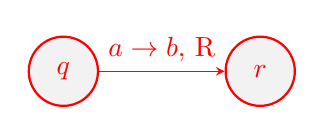
\begin{tikzpicture}
    \color{red}
        \node[state] (q_0) {$q$};
        \node[state, xshift=2.5cm] (r_0) {$r$};
    
        \draw
        (q_0) edge[] node[above]{$a \rightarrow b$, R}(r_0)
        ;
    \end{tikzpicture}
    \end{figure}\\
    Create transitions like this in $P$\\
        \begin{figure}[h]
    \centering
    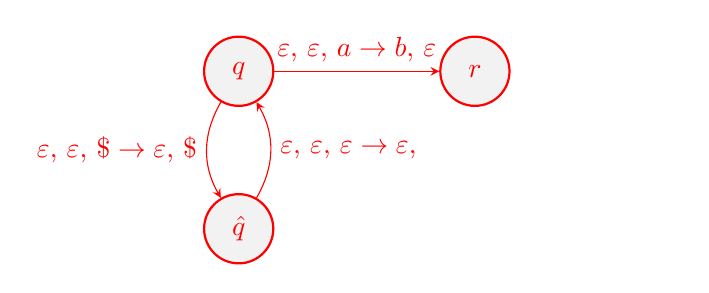
\begin{tikzpicture}
    \color{red}
        \node[state] (q_1) {$q$};
        \node[state, yshift=-2cm] (q) {$\hat{q}$};
        \node[state, xshift=3cm] (r_1) {$r$};
        \node[draw=none, xshift=5.5cm] (phantom) {};
        \draw
        (q_1) edge[] node[above]{$\e$, $\e$, $a \rightarrow b$, $\e$ }(r_1)
        (q_1) edge[bend right] node[left]{$\e$, $\e$, $\$ \rightarrow \e$, $\$$ }(q)
        (q) edge[bend right] node[right]{$\e$, $\e$, $\e \rightarrow \e$, \spc }(q_1)
        ;
    \end{tikzpicture}
    \end{figure}
    \item L transitions.\\
    For every transition of $M$ that looks like this\\
    \begin{figure}[h]
    \centering
    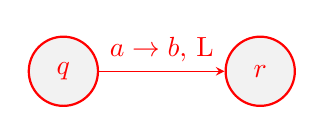
\begin{tikzpicture}
    \color{red}
        \node[state] (q_0) {$q$};
        \node[state, xshift=2.5cm] (r_0) {$r$};
    
        \draw
        (q_0) edge[] node[above]{$a \rightarrow b$, L}(r_0)
        ;
    \end{tikzpicture}
    \end{figure}\\
    Create transitions like this in $P$ $\forall c \in \s \cup \{$\spc$\}$ 
    \begin{figure}[h!]
    \centering
    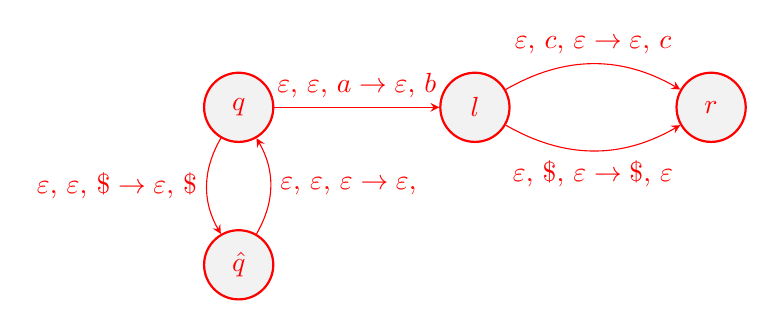
\begin{tikzpicture}
    \color{red}
        \node[state] (q_1) {$q$};
        \node[state, yshift=-2cm] (q) {$\hat{q}$};
        \node[state, xshift=3cm] (l) {$l$};
        \node[state, xshift=6cm] (r) {$r$};
        \draw
        (q_1) edge[] node[above]{$\e$, $\e$, $a \rightarrow \e$, $b$ }(l)
        (q_1) edge[bend right] node[left]{$\e$, $\e$, $\$ \rightarrow \e$, $\$$ }(q)
        (q) edge[bend right] node[right]{$\e$, $\e$, $\e \rightarrow \e$, \spc }(q_1)
        (l) edge[bend left] node[above]{$\e$, $c$, $\e \rightarrow \e$, $c$ }(r)
        (l) edge[bend right] node[below]{$\e$, $\$$, $\e \rightarrow \$$, $\e$ }(r)
        ;
    \end{tikzpicture}
    \end{figure}
\end{enumerate}
    \item [6.] $Q$ is the set of all the states we created.
    \begin{enumerate}
        \item The states from pre-processing $s$, $s_0$, $s_1$ and $s_2$.
        \item The states copied from the $M$.
        \item The new states $\hat{q}$ and $l$ defined by the transitions (for every transition).
    \end{enumerate}
\end{enumerate}
\end{quote}
}
\newpage
    \item [3.] [Exercise 2.6b] Write both a PDA and a CFG for the language
    \[
    L_3 = \overline{\{0^n1^n | n \geq 0\}}.
    \]
    For example, \str{000111} $\notin L_3$. Please include a brief explanation of why they work. (If you design a PDA and then convert it to a CFG, your explanation for the CFG can simply be, ``I converted my PDA to a CFG,'' and similarly if you convert a CFG to a PDA.)\newp
    Hint: First prove that this is equal to $\{0^m1^n| m \neq n\} \cup \overline{0^*1^*}$.\newp
    \answer{
Let $P$ be a $\mathcal{P}''$ program. Let us use the follow construction to create a Turing Machine $M$ that compiles $P$ into a standard single-tape TM.
\begin{quote}
\begin{enumerate}
    \item[i.] Initialize an empty stack to keep track of open loops.\footnote{At any point, if there is nothing to pop from this stack, $P$ was not a proper program. Additionally, if there are extra elements on the stack at the end, $P$ was not a proper program.}
    \item[ii.] Go through every character of the code and parse it in this way, keeping track of a counter $i$ for every character.\footnote{$i$ starts at 0, increments by 1 every time and $i,j \in \mathbb{Z}$} In the following steps, every transition created is from $q_i$ to $q_{i+1}$\\[2mm]
    \begin{tabular}{l l}
    \str{<} & $\forall j \in [0,n-1]$ Create transitions $a_j \rightarrow a_j$, L\\[2mm]
    \str{>} & $\forall j \in [0,n-1]$ Create transitions $a_j \rightarrow a_j$, R\\[2mm]
    \str{+} & $\forall j \in [0,n-2]$ Create transitions $a_j \rightarrow a_{j+1}$, S\\
    & Create transition $a_{n-1} \rightarrow a_0$, S\\[2mm]
    \str{-} & $\forall j \in [1,n-1]$ Create transitions $a_j \rightarrow a_{j-1}$, S\\
    & Create transition $a_{0} \rightarrow a_{n-1}$, S\\[2mm]
    \str{[} & Add $i$ to stack of open bracket placement.\\
    & $\forall j \in [1,n-1]$ Create transitions $a_{j} \rightarrow a_{j}$, S\\[2mm]
    \str{]} & Let $j$ be popped value from the open bracket placement stack.\\
    & Let $q_i$ = $q_j$ (create the looping state)\\
    & Create transition $a_{0} \rightarrow a_{0}$, S\\[2mm]
    \end{tabular}
    \item[iii.] $\forall q \in Q$ create a transition \spc\:$\rightarrow a_0, S$ from $q$ to itself.
    \item[iv.] Let $m$ be the length of the program $P$. $q_m$ is the final state that we have created so far. From $q_m$...
    \begin{itemize}
        \item $\forall j \in [1,n-1]$ create a transition $a_{j} \rightarrow a_{j}$, S to $q_{\text{\emph{accept}}}$.
        \item create a transition from $a_0 \rightarrow a_0$, S to $q_{\text{\emph{reject}}}$.
    \end{itemize}
\end{enumerate}
\end{quote}
The formal description of $M = \{Q, \s, \g, \delta, q_0,q_{\text{\emph{accept}}}, q_{\text{\emph{reject}}}\}:$
\begin{itemize}
    \item $Q = \{q_0,q_1...q_m,q_{\text{\emph{accept}}}, q_{\text{\emph{reject}}}\}$.
    \item $\s$ is a subset of $\g$ as defined by the directions without $a_0$ and \spc.
    \item $\g = \{a_0,...,a_{n-1},\text{\spc}\}$
    \item $\delta$ as defined above.
    \item $q_0$ as defined above.
    \item $q_{\text{\emph{accept}}}$ as defined above.
    \item $q_{\text{\emph{reject}}}$ as defined above.
\end{itemize}
}
\end{enumerate}
\end{document}